%!TEX root = ../thesis.tex

\chapter{Infrastructure}
\label{sec:infrastructure}

\todo[inline]{Still some overlap with the previous section. Need to make the distinction more clear. Diagrams in both sections could help to show that the “infrastructure” is a subset of the whole system.}

\todo[inline]{Maybe rename to Backend?}

The backend is the system subset related to sensor reading, thermostat control and data persistence.
%, i.e. the components the user does not directly interact with.
The terms infrastructure and backend are used synonymously in this section.
The infrastructure uses a server-client design pattern and is divided into the \emph{server} side and the \emph{local} side.
On the one hand, there is the server as an independent unit providing a public API to its clients allowing them to communicate and share their data.
On the other hand, there is the local deployment consisting of the installed wireless thermostats and the local communication gateway.
%The gateway uses the provided API to retrieve configuration from the server and populate it with data gathered from the deployed residential infrastructure.
Both sides will be explained in the following sections.
See Figure~\ref{fig:backend} for an overview.

\begin{figure}[h]
	\begin{center}
		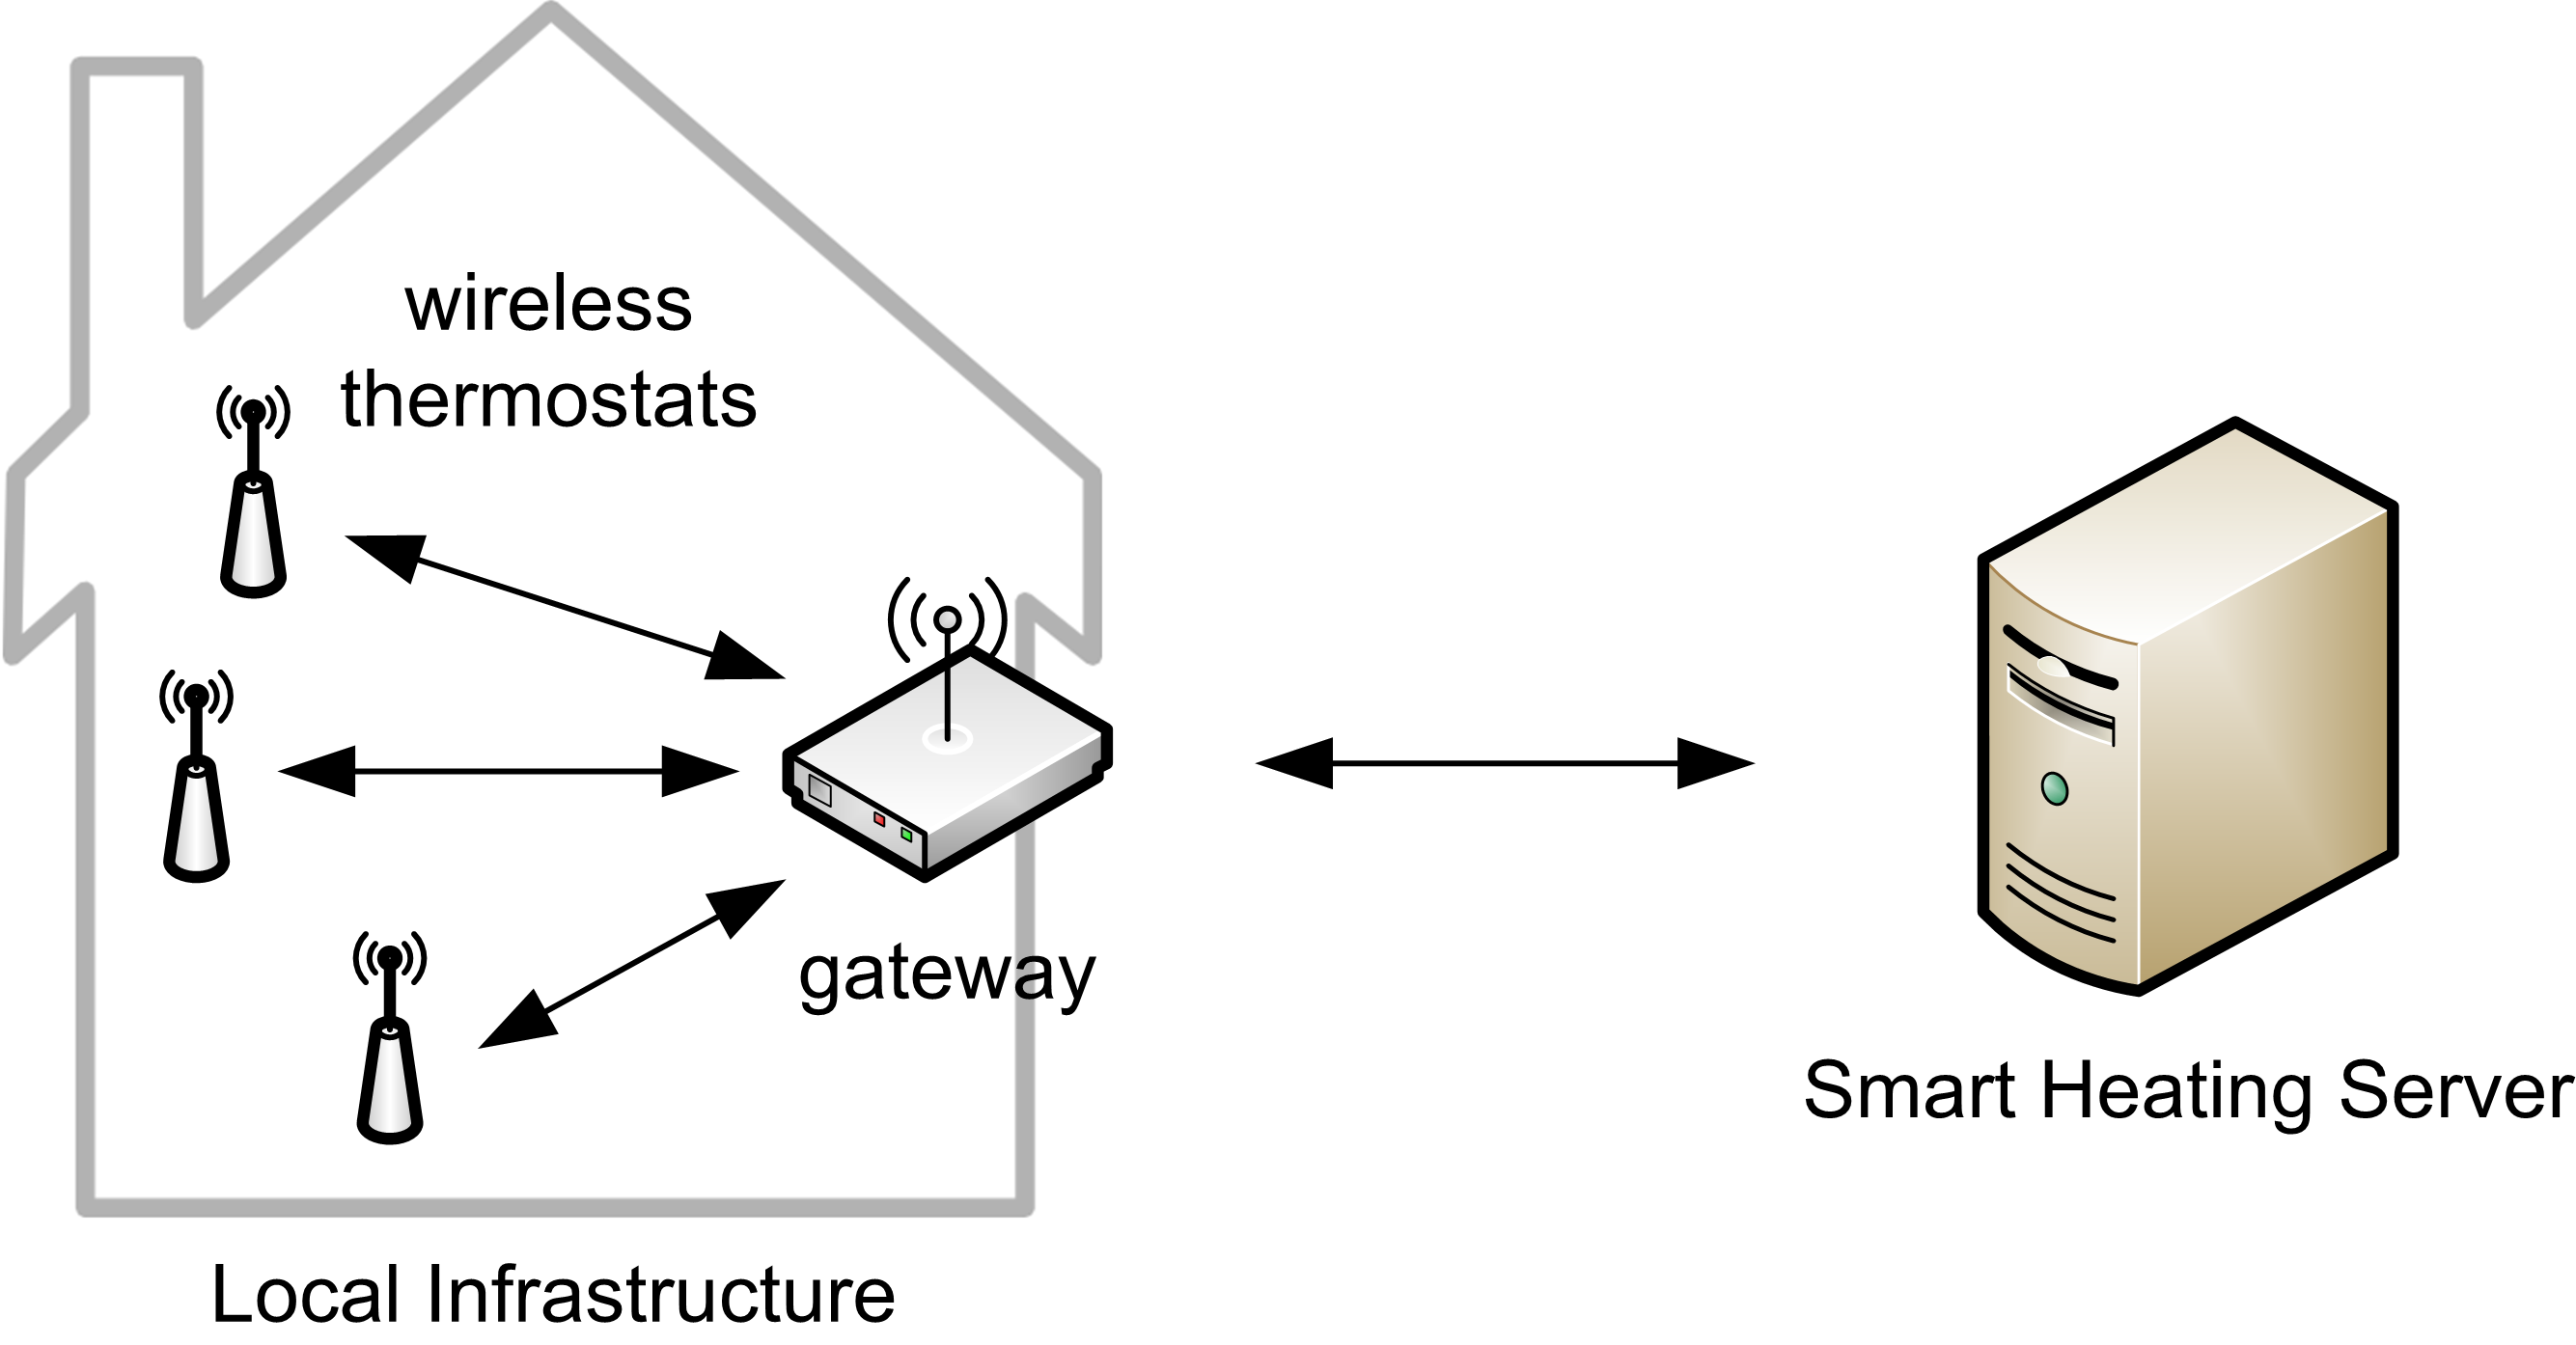
\includegraphics[width=0.8\textwidth]{images/Backend.png}
	\end{center}
	\caption{Overview of the backend consisting of the local deployment and the server infrastructure.}
	\label{fig:backend}
\end{figure}
